\section{Preferential attachment: \emph{"The rich get richer"}}
\label{sec:burstiness}

The term \textit{burstiness} describes the fact that some events appear in bursts, \textit{i.e.} once they appear, they are more likely to appear again. The notion of burstiness is similar to the one of aftereffect of future sampling \cite{feller_68}, which describes the fact that the more we observe an event, the higher the expectation to find new occurrences of this event. In (social) network studies, the burstiness effect is alos referred to as \textit{preferential attachment}\footnote{A.L. Barab\'asi, for example, uses the term \textit{preferential attachment} in \cite{barabasi1999emergence}, and \textit{burstiness} in \cite{barabasi_burst}.}: a node with many connections is more likely to have new connections than a node with few connections. To take into account this behavior, in the network generative model  (BA) \cite{albert2002statistical} model, a node is connected to an existing target node with a probability proportional to the number of links of the target node. This leads to scale-free networks that are characterized by a heavy tailed degree distribution, which can be approximated by a power law distribution such that the fraction of nodes $\pr(d)$ having a degree $d$ follows a power law $d^{-\gamma}$, where $\gamma$ typically ranges between 2 and 3~\cite{barabasi1999emergence}. 

Burstiness has been studied in different fields, in particular in computational linguistics and information retrieval to characterize word occurrences \cite{church1995poisson}. In these domains, simple definitions of burstiness, that directly capture the fact that a probability distribution is bursty if the probability of generating a new occurrences of an event increases with the number of occurrences of this event, have been proposed\cite{clinchant2008bnb,clinchant2010information}. We rely here on the discrete version of theses definitions, which takes the following form:
%
\begin{definition}[Burstiness]
	A discrete distribution $\pr$ is bursty if and only if, for all integers $(n, n')$, $n > n'$ :
	\begin{equation}
	\pr(X \geq n+1 \mid X \geq n) > \pr(X \geq n'+1 \mid X \geq n') \nonumber
	\end{equation}
	where $X$ denotes a random variable.
\label{def:burst}
\end{definition}
%
In the context of social networks, the notion of burstiness, or preferential attachment, appears at different levels: (a) a global preferential attachment level that characterizes the degree distribution of nodes in the network, (b) a local preferential attachment level that characterizes the degree distribution of nodes within communities, and (c) a feature burstiness level that characterizes the distributions of nodes among latent features. The feature burstiness characterize the importance of each features depending on how much they are represented within each nodes. We provide below a formal definition of these elements.
%


\begin{definition}[Burstiness in social networks]
Let $i$ be a node in a social network $G=(V,E)$, and let $d_i$ denote its degree. Furthermore, let $\mathcal{M} \in \{\M_e, \M_g\}$ be a link prediction model as defined in Section~\ref{sec:models}, and let $\Delta_n$ be the discrete differentiation on $n$: 
\begin{description}
\item[(i)] \emph{Global Preferential Attachment}: we say that $\mathcal{M}$ satisfies the global preferential attachment iff, for any node $i \in V$, we have:
 \begin{equation}
 \Delta_n \pr(d_i \geq n+1 | d_i \geq n,  \M) > 0
 \end{equation}
\item[(ii)] \emph{Local Preferential Attachment}: we say that $\mathcal{M}$ satisfies the local preferential attachment iff, for any node $i \in V$ and belonging to a community  $c$, we have:
  \begin{equation}
 \Delta_n \pr(d_{i,c} \geq n+1 | d_{i,c} \geq n,  \M) > 0
 \end{equation}
  Where $d_{i,c}$ denotes the degree of node $i$ in its community. \textcolor{red}{communities still ambiguous since we do not define it (moreover, we are in a context of soft clustering where node can belongs to several classes...)) }
\item[(iii)] \emph{Feature Burstiness}: we say that $\mathcal{M}_e$ satisfies the feature burstiness effect, iff, for any feature $k$ in the network,   
  \begin{equation}
	\Delta_n \pr(f_{\bm{.}k} \geq n+1 | f_{\bm{.}k} \geq n,  \M) > 0
  \end{equation}
   Where $f_{\bm{.}k}$ denotes the sum of the k-th features over all network's node such that $f_{\bm{.}k} = \sum_{j=0}^{N-1} f_{jk}$.
\end{description}
\label{def:burst-soc-net}
\end{definition}
%
The definitions of the different properties based on the burstiness involves inequalities whom are not easy to handle in general. Thus, we study in the following a way to formulate it in a more analytic and convenient form. Let us first define an appropriate random structure for exchangeable networks.

\begin{definition}
	Let $n$ and $N$ be two natural integer such that $N \geq n$. We define the random structure $x^{N,n}$ as a set of $N$ binary value having $n$ elements active (equal to one) and such that $\sum_{i=0}^N P(x^{N,i}) = 1$
	\label{def:rd_struct}
\end{definition}

This definition enables the link between the random variable $n$ being a integer (a node degree for example) and the structure that is homogeneous to a row (or a column) in a adjacency matrix that contains in some way this integer.

\begin{theorem}[Burstiness to Global Preferential Attachment] \label{th:burst_exch}
	 A degree distribution $p(d_i=n)$ of any node $i$ in a jointly exchangeable graph $G(V,E)$ is bursty iff :
	\begin{equation}
	 \Delta_n  p(y_{ij}=1 | d_i^{N,n}) \frac{N-n}{n+1} > 0
	\end{equation}

\end{theorem}

\begin{proof} 	\label{proof:glob}
	First we recall that for a jointly exchangeable graph, we have that:
	\begin{equation*}
	\p(y_{ij}: (i,j) \in V^2) = \p(y_{\sigma(i)\sigma(j)}: (i,j) \in V^2)
	\end{equation*}
	For any permutation $\sigma$ of the integer $\{1,..,n\}$. Furthermore it can be show that $ \pr(d_i \geq n'+1 \mid d_i \geq n')$ and $\frac{\p(d_i=n+1)}{\p(d_i=n)}$ vary in the same direction with $n$ (Clinchant 2006). Under the exchangeability assumptions, one can write that:
	
	\begin{align*}
	 b_n=\frac{\p(d_i=n+1)}{\p(d_i=n)} = \frac{\dbinom{N}{n+1} p(d_i^{N,n+1})}{\dbinom{N}{n} p(d_i^{N,n})}
	\end{align*}
 Applying a product rule, we have that:
	
	\begin{equation*}
	b_n = \frac{N-n}{n+1} \p(y_{ij}=1 | d_i^{N,n})
	\end{equation*}
	
	The differential is then equal to:
	\begin{align*}
	&\Delta_n b_n= b_{n+1} - b_n  \\
	&= \frac{N-n-1}{n+2} \p(y_{ij}=1 | d_i^{N,n+1}) - \frac{N-n}{n+1} \p(y_{ij}=1 | d_i^{N,n})
	\end{align*}
	
	The burstiness property is satisfied  $\forall n \in \mathbb{N}$ iff:
	\begin{align*}
	&\Delta_nb_n > 0 \iff \\
	& \frac{(n+1)(N-n-1)}{(n+2)(N-n)}\p(y_{ij}=1 | d_i^{N,n+1})  > \p(y_{ij}=1 | d_i^{N,n})
	\end{align*}
	\label{b-theorem}
\end{proof}
	
	The study of the series forming the left hand part of last equation gives hint about how and when the distribution $p$ would be bursty depending on the predictive distribution of one observation in the data. Particularly this series is less than one with a maxima at $(N-2)/2$ and is symmetric around this extrema for $N \in [0, N-2]$. We represent the series in figure \ref{fig:bp}.
	
	
	\begin{figure}[h]
		\centering
		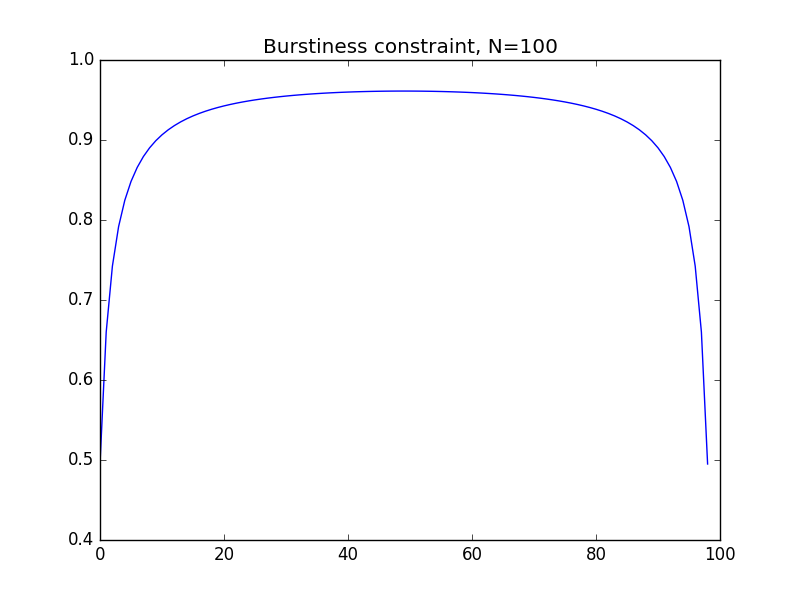
\includegraphics[scale=0.4]{img/bp}
		\caption{This plot represent the series that constraints the predictive distribution for the burstiness effect in exchangeable graph for N=100 (100 nodes)}
		\label{fig:bp}
	\end{figure}



Interestingly this theorem tell us how the burstiness effect, for exchangeable sequence with finite capacity $N$, will collapse for a small number of observation and notably, when the number of observations get closer to the capacity.\\

A typical form of the predictive distribution $\p(y_{ij}=1 | d_i^{N,n})$ is a linear function of the sufficient statistics of the observations (see \ref{prop:diaconis}). Though the burstiness effect would have specific constraint in this case.

We now study the case where the predictive distribution has a linear form such that:

\begin{equation}
p(y_{ij}=1 | d_i^{N,n}) = an+b
\end{equation}  
Where $n$ is a positive integers and $a$ and $b$ two positive real numbers. From theorem \ref{th:burst_exch} one has the following condition:

\begin{equation} \label{eq:polynom}
\frac{-an^2 -3an +a(N-1)-b(N+1)}{(n+2)(N-n)} > 0 
\end{equation}
The denominator of this equation is strictly positive for $n \in [0, N-1]$. The condition depend then on the sign of the numerator being a polynom of degree 2. Thus it admit 2 roots $n_-$ and $n_+$ such that:
\begin{align}
n_+ &= \frac{-3a + \sqrt{a(4N(a-b)+5a-4b)}}{2a} \\
n_- &= \frac{-3a - \sqrt{a(4N(a-b)+5a-4b)}}{2a} \\
\end{align}

If we study the polynom on the support of the real number, we can see that it is negative when $n$ tend to $+\infty$ and $-\infty$, thus the polynom take positive value between the roots if they exists. The condition of existence is:
\begin{equation}
a(4N(a-b)+5a-4b) > 0 \iff b < a \frac{4N+5}{4N+4}
\end{equation}

Furthermore, the roots need to be positive which traduce the following constraint:
\begin{align}
\sqrt{a(4N(a-b)+5a-4b)} > 3a \iff a\frac{N-1}{N+1} > b
\end{align}
If such constraint is satisfied, the polynom admit positive value for $n \in [0, n_+]$. This development shows that for certain form of the predictive distribution the burstiness can be satisfy for all integers $n$, but still a bursty phenomenon can exists on a subset which is determine by the hyperparameters of the model.

In particular let's suppose the predictive distribution take this specific form:
\begin{equation}
p(y_{ij}=1 | d_i^{N,n}) = \frac{n+\lambda_1}{N+\lambda_1+\lambda_0}
\end{equation}
This is equivalent to solving the polynom \eqref{eq:polynom} for $a=1$ and $b=\lambda_1$. In such a case, the burstiness effect will be present in the subset $n \in [0, n_+]$ iff the following holds:
\begin{equation}
\lambda_1 < \frac{N-1}{N+1}
\end{equation}

We now propose a relation to go from the definition of the local preferential effect to the predictive likelihood inside a latent class. The reason of why the theorem \ref{th:burst_exch} can not be directly applicable is because, when looking only at the relation that occur inside a class, one need to marginalize the remainder relation that are not in this class.

\begin{theorem}[Burstiness to Local Preferential Attachment] \label{th:burst_local}
	Let $\M_g$ be a network model of a jointly exchangeable graph $G(V,E)$ such that $f_i$ and $\phi_{kk'}$ are iid for any $i$, $k$ and $k'$.Moreover,  Let $N^c$ and $N^r$ be two integer such that the the former is the number of node in a class $c$, and the second the number of node not being in $c$, such that $N^c+N^r = N$. A local degree distribution $p(d_{i,c}=n)$ of any node $i$ in $c$ is bursty iif,
	
	\begin{equation}
\Delta_n  p(y_{ij}=1 | d_{i,c}^{N^c,n}) \frac{\sum_{r=0}^{N^r}\dbinom{N}{n+1+r} p(d_{ir}^{N^r,r})}{\sum_{r=0}^{N^r} \dbinom{N}{n+r} p(d_{ir}^{N^r,r}) } > 0
	\end{equation}
	
	
\end{theorem}

\begin{proof}
The exchangeable graph $G(V,E)$ contains $|V|=N$ nodes. Thus in the context of the local preferential attachment we consider the degree of a node $i$, in a class $c$ containing $N^c$ nodes and we denote the degree of this node within this class by $d_{i,c}$. We note the remaining number of node by $N^r = N - N_c$. We then write  distribution of the degree inside that class by marginalizing the possible edges between $i$ and the nodes that are not in $c$. We have:
\begin{equation}
p(d_{ic}=n) = \sum_{r=0}^{N^r} p(d_{ic}=n,d_{ir}=r)
\end{equation}
From exchangeable assumptions one as:

\begin{equation}
p(d_{ic}=n) = \sum_{r=0}^{N^r} \dbinom{N}{n+r} p(d_{ic}^{N^c, n},d_{ir}^{N^r, r})
\end{equation}
Under the assumptions that each local random parameters are i.i.d, we can separate the joint distribution: ( \textcolor{red}{on peut ouvrir la distribution avec les F et les Phi, pour voir que ca marche pour IMMSB mais pas pour ILFM, je me garde de l'écrire la pour gagner du temps !)}: 

\begin{align}
p(d_{ic}=n) &= \sum_{r=0}^{N^r} \dbinom{N}{n+r} p(d_{ic}^{N^c, n}) p(d_{ir}^{N_r, r}) \\
 &=  p(d_{ic}^{N^c, n})\sum_{r=0}^{N^r}   \dbinom{N}{n+r} p(d_{ir}^{N^r, r})
\end{align}

Finally by applying the burstiness properties as in proof \ref{proof:glob}, and product rule we can expess the burstiness in function of the predictive distribution:

\begin{equation} \label{eq:29}
b_n =  p(y_{ij}=1 | d_{i,c}^{N^c,n}) \frac{\sum_{r=0}^{N^r}\dbinom{N}{n+1+r} p(d_{ir}^{N^r,r})}{\sum_{r=0}^{N^r} \dbinom{N}{n+r} p(d_{ir}^{N^r,r}) }
\end{equation}

\end{proof}

\textcolor{red}{Open Probem:  Je n'ai pas encore réussi à solver le ratio ci-dessus permettant de conclure sur le local bursty}


We can see that in the case where $N^r=0$ equation \eqref{eq:29} reduce to:
\begin{equation}
b_n = p(y_{ij}=1 | d_{i,c}^{N^c,n}) \frac{\dbinom{N}{n+1}}{ \dbinom{N}{n+r} } =  p(y_{ij}=1 | d_{i,c}^{N^c,n}) \frac{N-n}{n=1}
\end{equation}

And in this case $N^c=N$. This show that the results of theorem \ref{th:burst_exch} and \ref{th:burst_local} are equivalent in this case which is sounds since $N^r=0$ means that there only one class, and so it is like evaluating the global preferential attachment.
%\begin{corollary}
%	A degree distribution  $p(d_i=n)$ of any node $i$ in a jointly exchangeable graph $G(V,E)$ such that it admits a predictive distribution of the form $\p(y_{ij}=1 | d_i^{N,n}) = an+b$, is bursty iff:
%Polynome solution, constraint on the positive roots, a, b > ...
%\end{corollary}

We now apply the previous results to characterize the preferential attachments effect in social networks.


\begin{proposition}
	The IMMSB models satisfy the local preferential attachments in the generative model $\M_g$. \textcolor{red}{No consensus yet on making this proposition on theorem V.1 or V.2 ? But theorem V.1 doesnt account for simulation that are always bursty with regards to the degree distribution}
\end{proposition}

\begin{proof}
In IMMSB one can write in the general case the predictive distribution conditioned by $d_i^{N,n}$:

\begin{equation} 
p(y_{ij} = 1 | d_i^{N,n}, \mathcal{M}_g) = \int_{\Theta} p(y_{ij}=1|\Theta) \frac{p(d_i^{N,n} | \Theta)}{p(d_i^{N,n})} p(\Theta) d\Theta \nonumber
\end{equation}

By only restraining the relations that occur inside class $c=\{k,k\}$, thus we note $N^c$ the total number of nodes being in the class $c$. In IMMSB being in class $c$ means that for an interaction between (any) nodes $i$ and $j$, they took membership associated to feature $k$.   (An other membership could be drawn for an other interaction, which make $N_c$ less or equal than $N$) . One can write the predictive distribution inside this class as follows:

\begin{align*} \label{eq:sum}
&p(y_{ij} = 1 | d_{ic}^{N^c,n}, \mathcal{M}_g)  \\
&=  \frac{ \int_{\phi_{c}} p(y_{ij}=1|\phi_{c}) p(d_{ic}^{N,n} | \phi_{c}) p(\phi_{c}) d\phi_{c}}{\int_{\phi_{c}} \p(d_{ic}^{N^c,n} | \phi_{c}))       p(\phi_{c}) d\phi_{c}}   \\
&= \frac{\int_{\phi_c} \phi_c^{n+1}(1-\phi_c)^{N^c-n} \phi_c^{\lambda_1-1} (1-\phi_c)^{\lambda_0-1} d\phi_{c}}{\int_{\phi_c} \phi_c^{n}(1-\phi_c)^{N^c-n} \phi_c^{\lambda_1-1} (1-\phi_c)^{\lambda_0-1} d\phi_{c}} \\
&= \frac{ \text{B}(n+1+\lambda_1, N^c-n+\lambda_0) }{\text{B}(n+\lambda_1, N^c-n+\lambda_0)} \\
&= \frac{n+\lambda_1}{N^c + \lambda_1 +\lambda_0}
\end{align*}

Where $\text{B}()$ is the beta function. The last equation show that the predictive likelihood is strictly crescent with $n$.

\end{proof}

\begin{proposition}
	The ILFM model does not satisfy the local preferential attachments in the generative model $\M_g$.
\end{proposition}

\begin{proof}
As for IMMSB proof, we only consider the relations  that occur inside class $c=\{k,k\}$, thus we note $N^c$ the total number of nodes being in the class $c$. In ILFM being in the class $c$ means that we evaluate the predictive distribution by only considering the column $k$ of the feature matrix. We can interpret this operation has looking the connections pattern when only the contribution of the feature $k$ is at work. One can write the predictive distribution inside this class as follows:

\begin{align*}
&\p(y_{ij}=1 | d_{ic}^{N^c,n}, \M_g)  \\
&=  \frac{ \int_{\phi_{c}} p(y_{ij}=1|\phi_{c}) p(d_{ic}^{N,n} | \phi_{c}) p(\phi_{c}) d\phi_{c}}{\int_{\phi_{c}} \p(d_{ic}^{N^c,n} | \phi_{c}))       p(\phi_{c}) d\phi_{c}} \\
&= \frac{ \int_{\phi_{c}} \sigma(\phi_c) \sigma(\phi_c)^n (1-\sigma(\phi_c))^{N^c-n}     p(\phi_{c}) d\phi_{c}}{\int_{\phi_{c}}  \sigma(\phi_c)^n (1-\sigma(\phi_c))^{N^c-n}      p(\phi_{c}) d\phi_{c}} \\
&= \frac{ \int_{\phi_{c}} \sigma(\phi_c) \sigma(\phi_c)^n \sigma(-\phi_c)^{N^c-n}     p(\phi_{c}) d\phi_{c}}{\int_{\phi_{c}}  \sigma(\phi_c)^n \sigma(-\phi_c)^{N^c-n}      p(\phi_{c}) d\phi_{c}} \\
&= \frac{ \int_{\phi_{c}} \sigma(\phi_c) (\frac{\sigma(\phi_c)}{\sigma(-\phi_c)})^n \sigma(-\phi_c)^{N^c}     p(\phi_{c}) d\phi_{c}}{\int_{\phi_{c}}  (\frac{\sigma(\phi_c)}{\sigma(-\phi_c)})^n \sigma(-\phi_c)^{N^c}     p(\phi_{c}) d\phi_{c}} \\
&= \frac{ \int_{\phi_{c}} \frac{\exp(n\phi)}{1+\exp(-\phi)} \frac{\exp(-N\phi)}{(1+\exp(-\phi))^{N^c}}  p(\phi_{c}) d\phi_{c}}{\int_{\phi_{c}}  \exp(n\phi) \frac{\exp(-N\phi)}{(1+\exp(-\phi))^{N^c}}   p(\phi_{c}) d\phi_{c}} \\
&= \frac{ \int_{\phi_{c}} \exp(\phi(n-N)) \sigma(\phi)^{N+1} p(\phi_{c}) d\phi_{c}}{\int_{\phi_{c}} \exp(\phi(n-N)) \sigma(\phi)^{N} p(\phi_{c}) d\phi_{c}} \\
\end{align*}

With $\sigma(\phi) = \frac{1}{1+\exp(-\phi)}$ and $\p(\phi) = \mathcal{N}(0, \sigma_w)$.


\textcolor{red}{not ended yet...no theorem to go from the definition to the predictive likelihood}
\end{proof}

\begin{proposition}
	The ILFM and IMMSB models do not satisfy the global and local preferential attachments. in the mode $\M_e$.
\end{proposition}

The proof of this statement is trivially true in the sens that given $\mat{F}$ and $\mat{\Theta}$, the likelihood is fully determined and hence do not depend on new links being generated. More precisely one has:
\begin{align}
\p(y_{ij}=1| d_i^{N,n}, \M_e) &= \p(y_{ij}=1| \M_e)\\
&= \mat{\hat{f}}_{i} \mat{\hat{\Phi}} \mat{\hat{f}}_j^\top
\end{align}
The predictive likelihood does not depend on $n$, and it follows from theorem \ref{th:burst_exch} that the burstiness is not satisfied in this case (specifically because the series $\frac{N-n}{n+1}$ is decreasing for $n\in [0, N-2]$).

Furthermore, we show simulations, where figure \ref{fig:gen_burst_mmsb} show some complex pattern in the empirical distribution of the overall degree that are clearly non bursty. One can note that, despite this result, the inference procedure of the posterior distribution will be likely to produce latent features that fit an possible presence of burstiness of the data. This is particularly visible on the predictive likelihood for IMMSB which take the following form (see details in appendix \ref{sec:append}):
\begin{equation} \label{eq:ppp}
p(y_{ij}=1 | \M_e)\propto \sum_{kk'} \frac{M_{(kk')1} + \lambda_1}{M_{(kk')\bm{.}} + \lambda_0 + \lambda_1}  (N_{ik} + \alpha\beta_k ) (N_{jk} + \alpha\beta_k)
\end{equation}   
One can see the features that are associated with the weights that cumulate number of observed links will be likely to generate links. In the case of ILFM the mixing between feature and weight is less clear since the non-conjugacy produce no close relation between the posterior and the sufficient statistics of the data (ie the degrees count). 

The same development holds for the local burstiness by selecting the appropriate class in the summation of equation \eqref{eq:ppp}.
\begin{proposition} \label{prop:diaconis}
	Both ILFM and IMMSB models satisfy the feature burstiness for $n < L$ under some conditions on their hyperparameters  and $L$ a number of observation depending of the hyperparameters.
\end{proposition}

\begin{proof}
The Diaconis-Ilvisaker theorem \cite{diaconis1979conjugate} state \emph{'subject to regularity conditions, the conjugate priors typically used satisfy, and are characterized by, a  similar relation of posterior linearity'}:
\begin{equation}
\E_\Theta[\E_{X|\Theta}[X\mid \Theta] \mid X=x] = ax+b \quad \text{for} \quad x=0,1,2,... \nonumber
\end{equation}

Especially, the Dirichlet Process and the Indian Buffet Process, as prior for the latent features, are typically build on the suitable conjugate distribution respectively Dirichlet-Multinomial and Beta-Bernoulli. Furthermore, this claim is highlighted by the Gibbs update that corroborate the feature burstiness effect:
\begin{align} \label{eq:feat_up}
&\p(f_{ik} = 1 | F^{-ik}) = \frac{m_k^{-ik}}{N} \qquad \text{ILFM feature update} \nonumber \\
&\p(f_{ik} = 1 | F^{-ik}) = \frac{n_{ik}^{-z_{ij}}+\alpha_k}{N+\alpha_.} \qquad \text{IMMSB feature update} \nonumber \\
\end{align}

Where the $m_k^{-ik}$ described the number of elements that have the $k$-iem feature active except for element $i$, similarly $n_{ik}^{-z_{ij}}$ represents the number of times that $i$ was assigned to $k$ except for relation $(ij)$ (class membership are jointly sampled in MMSB).

By applying theorem \ref{th:burst_exch} for linear predictive distribution, it can be easily show that the burstiness is true below a number $L$ which is the positive roots of the polynom:
\begin{equation}
	 an^2 + 3an - a(N-1) + b(N+1) = 0
\end{equation}

The condition on the hyperparameters $a$ and $b$ arise in order to find a strictly positive roots of this polynom. In the case of ILFM and IMMSB, it is equivalent to solve the polynom with a=1 and  $b=0$ or $b=\alpha_k$ for respectively ILFM and IMMSB. The positive roots arise in this case if $b < 1$, which determines $L$.
\end{proof}

We represent tree networks generated by ILFM in figure \ref{fig:gen_burst_ilfm} and IMMSB \ref{fig:gen_burst_mmsb}. We compute a goodness of fit to quantify the power law hypothesis on the empirical degree distributions. The protocol is described in section \ref{sec:experiments-busrt}. As an empirical illustration for our claims on preferential attachment, we show a 3*3 figure where each columns is particular setting of hyper-parameter and the rows are respectively, the global degree distribution, the local degree distribution and feature distribution (on a max a assignment point of view).

As we can see in the experiments, we can generate networks that do not fit the burstiness definition on the overall degree distribution.

\begin{figure}[h]
	\centering
	
	\minipage{0.16\textwidth}
	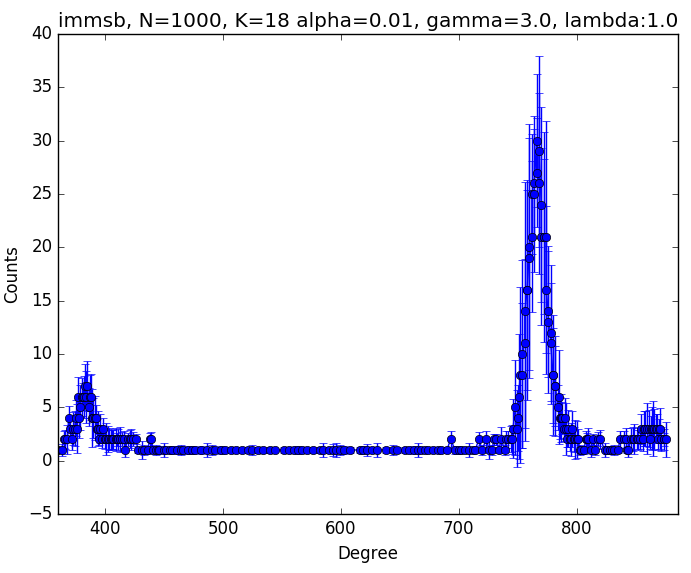
\includegraphics[width=3.2cm, height=3.7cm]{img/M_g_peaks/figure_1}
	\endminipage
		\minipage{0.16\textwidth}
	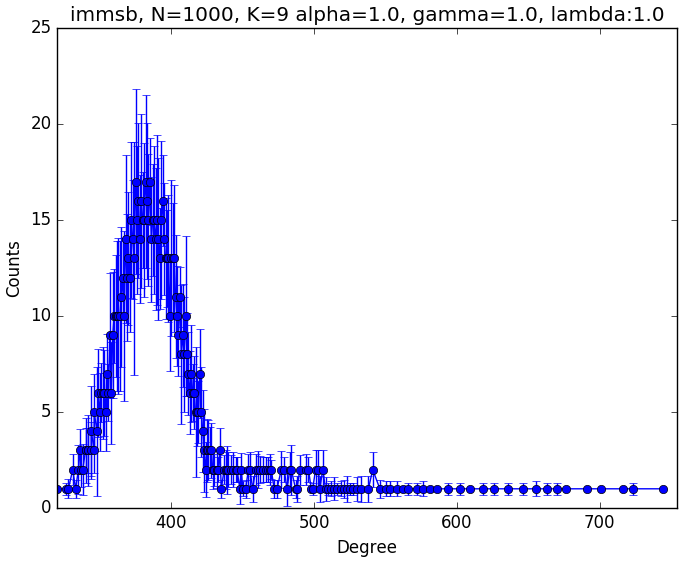
\includegraphics[width=3.2cm, height=3.7cm]{img/M_g_power_law/figure_1}
	\endminipage
	\minipage{0.16\textwidth}
	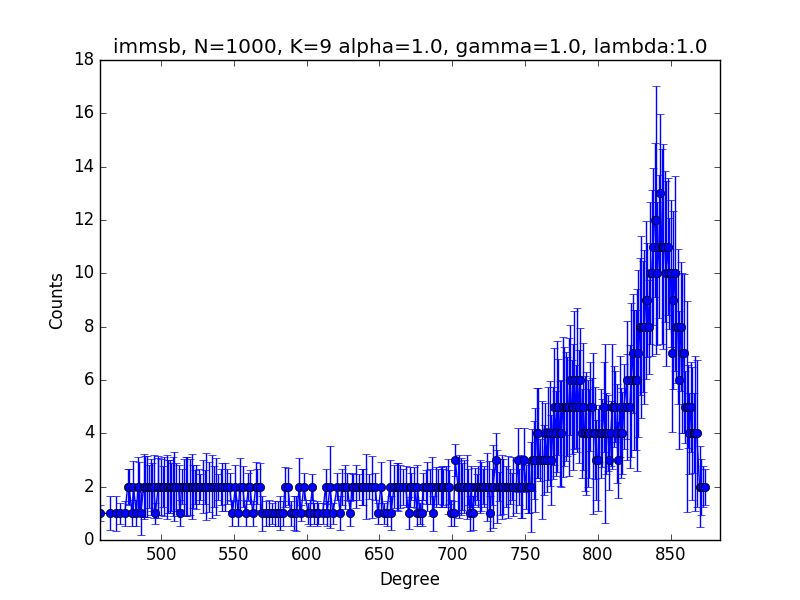
\includegraphics[width=3.2cm, height=3.7cm]{img/M_g_regular/figure_1}
	\endminipage
		\vspace{-0.4cm}
	\minipage{0.16\textwidth}
	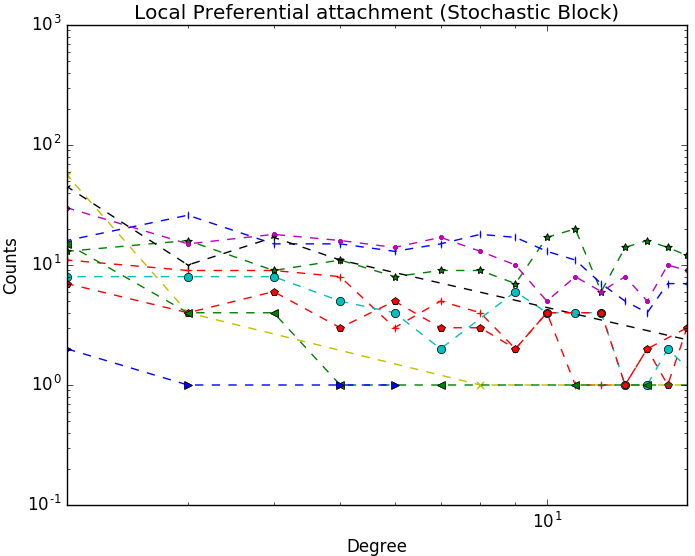
\includegraphics[width=3.2cm, height=3.7cm]{img/M_g_peaks/figure_3}
	\endminipage
		\minipage{0.16\textwidth}
	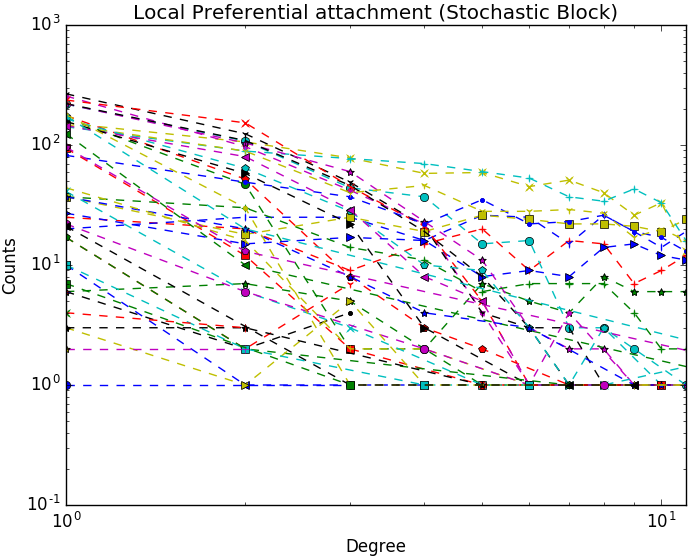
\includegraphics[width=3.2cm, height=3.7cm]{img/M_g_power_law/figure_3} 
	\endminipage
	\minipage{0.16\textwidth}
	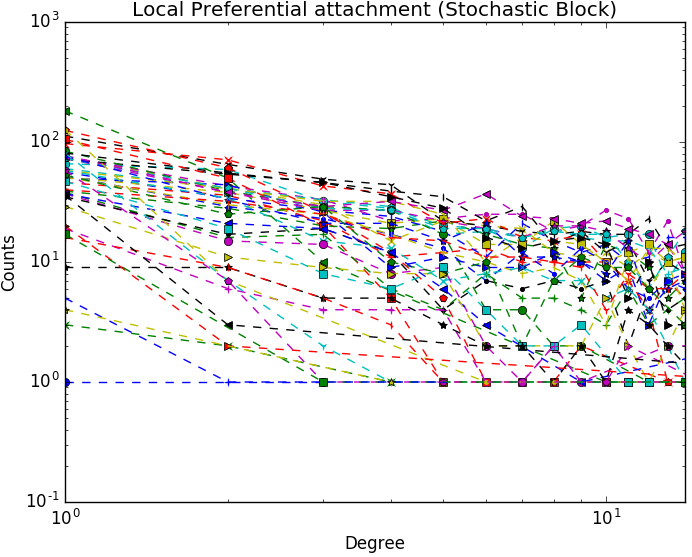
\includegraphics[width=3.2cm, height=3.7cm]{img/M_g_regular/figure_3}
	\endminipage
		\vspace{-0.4cm}
	\minipage{0.16\textwidth}
	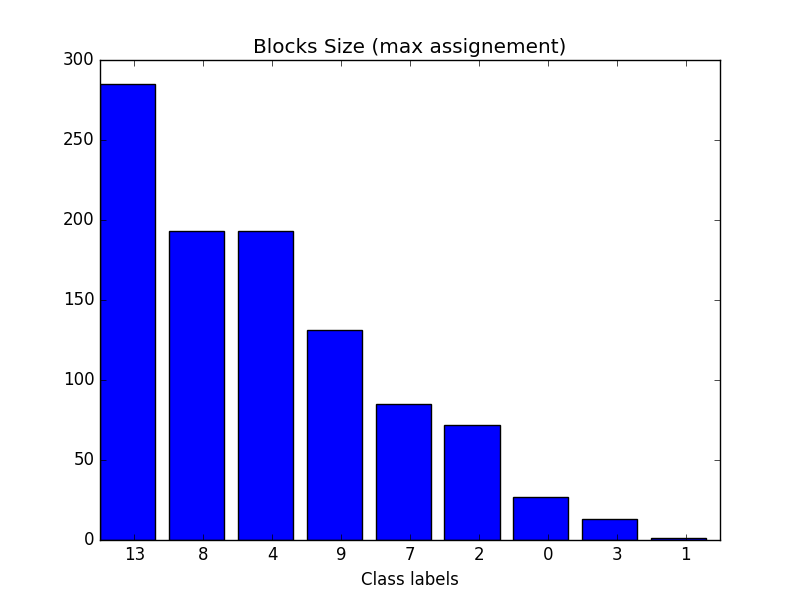
\includegraphics[width=3.2cm, height=3.7cm]{img/M_g_peaks/figure_5}
	\endminipage
	\minipage{0.16\textwidth}
	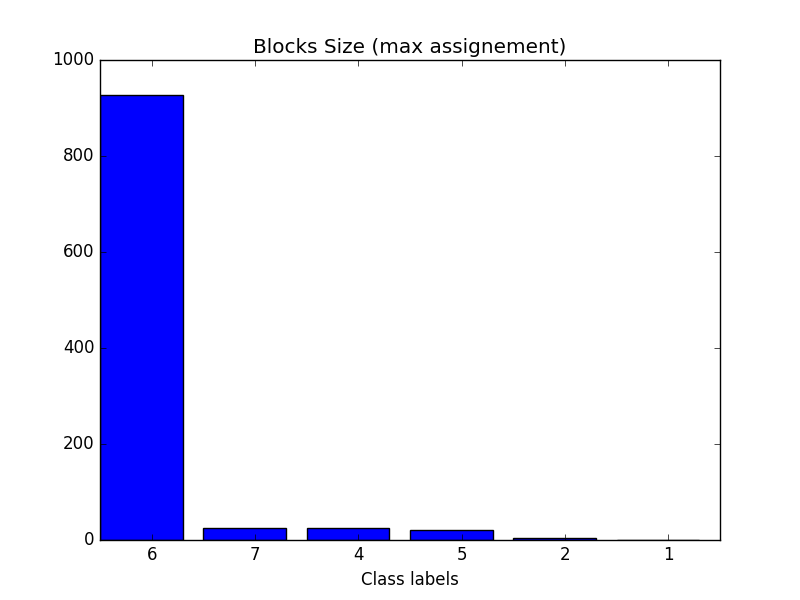
\includegraphics[width=3.2cm, height=3.7cm]{img/M_g_power_law/figure_5} 
	\endminipage
	\minipage{0.16\textwidth}
	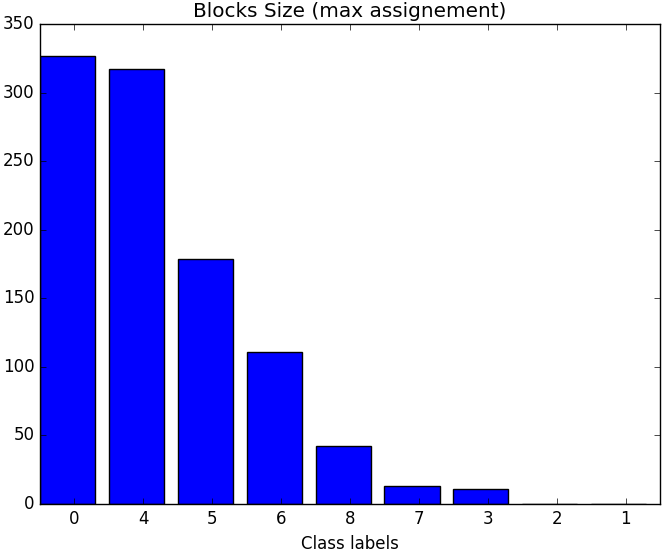
\includegraphics[width=3.2cm, height=3.7cm]{img/M_g_regular/figure_5}
	\endminipage
	\caption{Generated Networks with in three different settings (same set than for figure \ref{fig:gen_blocks}). The upper figures show the global preferential attachment. The lower figures show the local preferential attachment. While global preferential attachment is not a pure features of model, we see that the local preferential attachment has linear form in the log-log space.}
	\label{fig:gen_burst_mmsb}
\end{figure}



